\documentclass[12pt]{beamer}
%\documentclass[20pt,handout]{beamer}
\usetheme{Darmstadt}
\usepackage{graphicx}
%\usepackage[german]{babel}
\usepackage{ngerman}
\usepackage[T1]{fontenc}
\usepackage[utf8]{inputenc}
\usepackage{tikz}
\setbeamertemplate{footline}[frame number]

\newcommand{\cc}[1]{\includegraphics[height=4mm]{img/#1.png}\hspace{1mm}}
\usepackage{ifthen}
\newcommand{\license}[2][]{\\#2\ifthenelse{\equal{#1}{}}{}{\\\scriptsize\url{#1}}}
\usepackage{textcomp}
\usepackage{hyperref}

\pgfdeclareimage[height=.6cm]{c3d2logo}{./img/c3d2.pdf}


\pgfdeclarelayer{foreground}
\pgfsetlayers{main,foreground}
\logo{\pgfputat{\pgfxy(-1,0)}{\pgfbox[center,base]{\pgfuseimage{c3d2logo}}}}


\title{Datenschutz und Datensicherheit}
\author{\small Stephan Thamm\\\large Chaos Computer Club Dresden}
\date{10.11.2016}

\begin{document}
\maketitle

\section{Einleitung}
\subsection{}

\begin{frame}
  \frametitle{Chaos Computer Club}
  \begin{figure}
    \includegraphics[height=0.7\textheight]{img/fingerabdruck.jpg}
  \end{figure}
\end{frame}

\begin{frame}
    \frametitle{Chaos Computer Club}
    \begin{center}
	\includegraphics[height=0.2\textheight]{img/chaosknoten.png}
    \end{center}	
    \begin{itemize}
      \item<1-> Verein wurde 1981 gegr"undet (\url{https://ccc.de})          
      \item<2-> Aktuell mehr als 6000 Mitglieder
      \item<3-> Betreibt u.a. "Offentlichkeitsarbeit und Politikberatung      
      \item<4-> Lokale Erfahrungsaustauschkreise (Erfas) und Chaostreffs
    \end{itemize}
\end{frame}

\begin{frame}
  \frametitle{Chaos Computer Club Dresden}
  \begin{center}
    \includegraphics[height=0.1\textheight]{img/c3d2_logo.png}
  \end{center}
  \begin{itemize}
    \item<1-> Chaos Computer Club Dresden (\url{https://c3d2.de})          
    \item<2-> Datenspuren (\url{https://datenspuren.de})
    \item<3-> Radio und Podcasts (\url{https://c3d2.de/radio.html})
    \item<4-> Chaos macht Schule (\url{https://c3d2.de/schule.html})
  \end{itemize}
\end{frame}

\begin{frame}
  \frametitle{Stasi vs. NSA}
  \begin{center}
    \only<1> {
      \begin{center}
        ``Wir wissen z.B., dass es nicht so ist, wie bei der Stasi und dem KGB, dass es dicke Aktenbände gibt, wo unsere Gesprächsinhalte alle aufgeschrieben und schön abgeheftet sind. Das ist es nicht.'' \\
        (Gauck, 30.06.2013 im ZDF-Sommerinterview)
      \end{center}
    }
    \only<2>{
      \includegraphics[height=0.7\textheight]{img/akten1.png}
    }
    \only<3>{
      \includegraphics[height=0.7\textheight]{img/akten2.png}
    }
  \end{center}
\end{frame}

\section{Geheimdienste}
\subsection{}

\begin{frame}
    \frametitle{NSA-Skandal}
    \begin{center}
      \includegraphics[height=0.7\textheight]{img/snowden.jpg}
    \end{center}	
\end{frame}

\begin{frame}
  \frametitle{Internet}
  \begin{center}
    \only<1>{
      \includegraphics[height=0.7\textheight]{img/internet_0.jpg}
    }
    \only<2>{
      \includegraphics[height=0.7\textheight]{img/internet_2.jpg}
    }
    \only<3>{
      \includegraphics[height=0.6\textheight]{img/internet_1.png}
    }
  \end{center}
\end{frame}

\begin{frame}
    \frametitle{Tempora}
    \includegraphics[height=0.7\textheight]{img/spiegel-tempora.png}
\end{frame}

\begin{frame}
    \frametitle{Beispiel Mail}
    \begin{center}
      \includegraphics[height=0.7\textheight]{img/telekom_mail.png}
    \end{center}	
\end{frame}

\begin{frame}
    \frametitle{Kindernet}
    \pause
    \includegraphics[height=0.7\textheight]{img/kindernet.png}
\end{frame}

\begin{frame}
    \frametitle{Prism}
    \pause
    \begin{center}
      \includegraphics[height=0.7\textheight]{img/prism.jpg}
    \end{center}
\end{frame}

\begin{frame}
  \frametitle{Verhaltensänderung}
  \begin{center}
    \includegraphics[height=0.7\textheight]{img/verhalten.png}
  \end{center}
\end{frame}

\begin{frame}
    \frametitle{``Ich habe ja nichts zu vergergen''}
    \pause
    \begin{center}
      ``Arguing that you don't care about the right to privacy because you have nothing to hide is no different than saying you don't care about free speech because you have nothing to say. ''
      (Edward Snowden, 21.05.2015 auf Reddit)
    \end{center}
\end{frame}

\section{Metadaten}
\subsection{}

\begin{frame}
  \frametitle{Metadaten}
  \only<2>{
    \begin{center}
      \fbox{
        \includegraphics[height=0.7\textheight]{img/psb.png}
      }
    \end{center}
  }
  \only<3>{
    \begin{center}
      \large Metadaten oder Metainformationen sind Daten, die Informationen über Merkmale anderer Daten enthalten, aber nicht diese Daten selbst.
    \end{center}
  }
\end{frame}

\begin{frame}
  \frametitle{Vorratsdatenspeicherung}
  \begin{itemize}
    \item<2-> Standortdaten der Teilnehmer aller Mobiltelefonate bei Beginn des Telefonats, zu speichern für 4 Wochen
    \item<3-> Standortdaten bei Beginn einer mobilen Internetnutzung, zu speichern für 4 Wochen
    \item<4-> Rufnummern, Zeit und Dauer aller Telefonate, zu speichern für 10 Wochen
    \item<5-> Rufnummern, Sende- und Empfangszeit aller SMS-Nachrichten, zu speichern für 10 Wochen
    \item<6-> zugewiesene IP-Adressen aller Internetnutzer sowie Zeit und Dauer der Internetnutzung, zu speichern für 10 Wochen
  \end{itemize}
\end{frame}

\begin{frame}
  \frametitle{Verbindungsdaten}
  \begin{center}
    \only<1>{
      \includegraphics[height=0.7\textheight]{img/metadaten_studie.png}
    }
    \only<2>{
      \includegraphics[height=0.7\textheight]{img/metadata-matters.jpg}
    }
  \end{center}
\end{frame}

\begin{frame}
  \frametitle{Bewegungsdaten}
  \pause
  \begin{center}
    \includegraphics[height=0.7\textheight]{img/maltespitz.png}
  \end{center}
\end{frame}

\begin{frame}
  \frametitle{Telefonica}
  \pause
  \begin{center}
    \includegraphics[height=0.7\textheight]{img/telefonica.png}
  \end{center}
\end{frame}

\begin{frame}
	\frametitle{Google Takeout}
  \begin{center}
    \only<2>{
      \includegraphics[height=0.4\textheight]{img/google_heat_1.png}
    }
    \only<3>{
      \includegraphics[height=0.4\textheight]{img/google_heat_2.png}
    }
  \end{center}
\end{frame}

\begin{frame}
	\frametitle{Datenanalyse - Zeit}
  \begin{center}
    \only<2>{
      \includegraphics[height=0.4\textheight]{img/punch_1.png}
    }
    \only<3>{
      \includegraphics[height=0.4\textheight]{img/punch_2.png}
    }
    \only<4>{
      \includegraphics[height=0.4\textheight]{img/punch_3.png}
    }
  \end{center}
\end{frame}

\begin{frame}
  \frametitle{Was tun die USA mit Metadaten?}
  \begin{center}
    \only<2>{
      \includegraphics[height=0.7\textheight]{img/wekillpeople.jpg}
    }
    \only<3>{
      \includegraphics[height=0.7\textheight]{img/terminator.jpg}
    }
    \only<4>{
      \includegraphics[height=0.7\textheight]{img/skynet.png}
    }
    \only<5>{
      \includegraphics[height=0.7\textheight]{img/skynet2.png}
    }
  \end{center}
\end{frame}

\section{Wirtschaft}
\subsection{}

\begin{frame}
  \frametitle{Firmen}

  \begin{itemize}
    \item<2-> Womit verdienen folgende Firmen ihr Geld?
      \begin{itemize}
        \item<3-> Karstadt
        \item<4-> Amazon
        \item<5-> Ebay
        \item<6-> Facebook
      \end{itemize}
  \end{itemize}
\end{frame}

\begin{frame}
  \frametitle{Gesch"aftsmodelle}
  \begin{figure}
    \includegraphics[height=0.7\textheight]{img/business_pigs.jpg}
  \end{figure}
\end{frame}

\begin{frame}
  \frametitle{Soziale Netzwerke}

  \begin{itemize}
    \item Was haben soziale Netzwerke von ihren Nutzen?\\(am Bsp. von Facebook)
      \begin{itemize}
        \item<2-> 82\% Einnahmen aus Werbung
        \item<3-> 30\% Anteil an "`Facebook-Einkäufen"'
        \item<4-> durchschnittlich 1€/Profil
        \item<5-> "`Poweruser"'-Profile deutlich mehr
        \item<6-> => Mehr Werbegewinn durch personalisierte Werbung
        \item<7-> Q2 2014 791 Mio Dollar Gewinn
      \end{itemize}
  \end{itemize}
\end{frame}

\begin{frame}
  \frametitle{Wert von Daten}
  \pause
  \begin{center}
    \includegraphics[height=0.7\textheight]{img/jim_verkaufen.png}
  \end{center}
\end{frame}

\begin{frame}
  \frametitle{Lock in effect}
  \begin{center}
    ``Tie all of our products together, so we further lock customers into our ecosystem'' (Steve Jobs)
  \end{center}
\end{frame}

\begin{frame}
  \frametitle{Werbenetzwerke}
  \begin{center}
    \only<1>{
      \includegraphics[height=0.3\textheight]{img/lightbeam_0.png}
    }
    \only<2>{
      \includegraphics[height=0.7\textheight]{img/lightbeam_1.png}
    }
    \only<3>{
      \includegraphics[height=0.7\textheight]{img/lightbeam_2.png}
    }
    \only<4>{
      \includegraphics[height=0.7\textheight]{img/lightbeam_3.png}
    }
    \only<5>{
      \includegraphics[height=0.7\textheight]{img/disconnect.png}
    }
  \end{center}
\end{frame}

\begin{frame}
  \frametitle{Gezielte Werbung}
  \pause
  \begin{center}
    \includegraphics[height=0.8\textheight]{img/pregnant.png}
  \end{center}
\end{frame}

\begin{frame}
  \frametitle{Datensparsamkeit}
  \begin{itemize}
    \item<2-> Vermeidung von Daten
    \item<3-> Vermeidung von echten Daten
    \item<4-> Pseudonymisierung
    \item<5-> Auswahl von Diensten, Software und Hardware
    \item<6-> Abwägung von Nutzen und Kosten
  \end{itemize}
\end{frame}

\section{Soziales}
\subsection{}

\begin{frame}
  \frametitle{Das Internet vergisst nicht}
  \begin{itemize}
    \item<2-> Recht auf Vergessen?
    \item<3-> alle Daten sind Kopien
    \item<4-> keinerlei Kontrolle über Verarbeitung
    \item<5-> archive.org
  \end{itemize}
\end{frame}

\begin{frame}
  \frametitle{Datenschutz anderer Personen}
  \begin{itemize}
    \item<2-> Erwähnung in Kommentaren, Tweets etc
    \item<3-> Veröffentlichung Bilder
    \item<4-> ''No pics, so it didn't happen''
    \item<5-> Importieren von Kontaktdaten
  \end{itemize}
\end{frame}

\begin{frame}
  \frametitle{Cybermobbing}
  \pause
  \begin{center}
    \large{Keine technische Lösung für soziale Probleme}
  \end{center}
\end{frame}

\section{Urheberrecht}
\subsection{}

\begin{frame}
  \frametitle{Urheberrechtsverletzungen}
  \begin{itemize}
    \item<2-> Konsument oder Anbieter?
    \item<3-> Störerhaftung
    \item<4-> Nutzungsvereinbarung
    \item<5-> Änderung des Telemediengesetzes
  \end{itemize}
\end{frame}

\begin{frame}
  \frametitle{Recht am eigenen Bild}
  \pause
  \begin{center}
    \large{Einverständniserklärung}
  \end{center}
\end{frame}

\begin{frame}
  \frametitle{Freie Lizenzen}
  \pause
  \begin{center}
    \includegraphics[height=0.4\textheight]{img/creative_commons.png}
  \end{center}
\end{frame}

\section{Gegenmaßnahmen}
\subsection{}

\begin{frame}
  \frametitle{Verständnis für die Technik}
  \begin{center}
    \only<2>{
      \includegraphics[height=0.7\textheight]{img/pentabug.jpg}
    }
    \only<3>{
      \includegraphics[height=0.7\textheight]{img/raspberry_pi.png}
    }
  \end{center}
\end{frame}

\begin{frame}
    \frametitle{Passwörter}
    \begin{itemize}
        \item<2-> Keine einfachen Wörter
        \item<3-> Groß-, Kleinbuchstaben, Ziffern, Sonderzeichen
        \item<4-> Beispiele:
            \begin{itemize}
                \item<5-> dragon
                \item<6-> (nCuAj.§Tsm!f
                \item<7-> IchLiebeDich
                \item<8-> .§)=)=`
                \item<9-> 123456
                \item<10-> qwerty
                \item<11-> Mks?o/.u,1Psw!
            \end{itemize}
        \item<12-> Verschiedene Passwörter nutzen!
    \end{itemize}
\end{frame}

\begin{frame}
    \frametitle{Verschlüsselung: symmetrisch}
    \begin{center}
	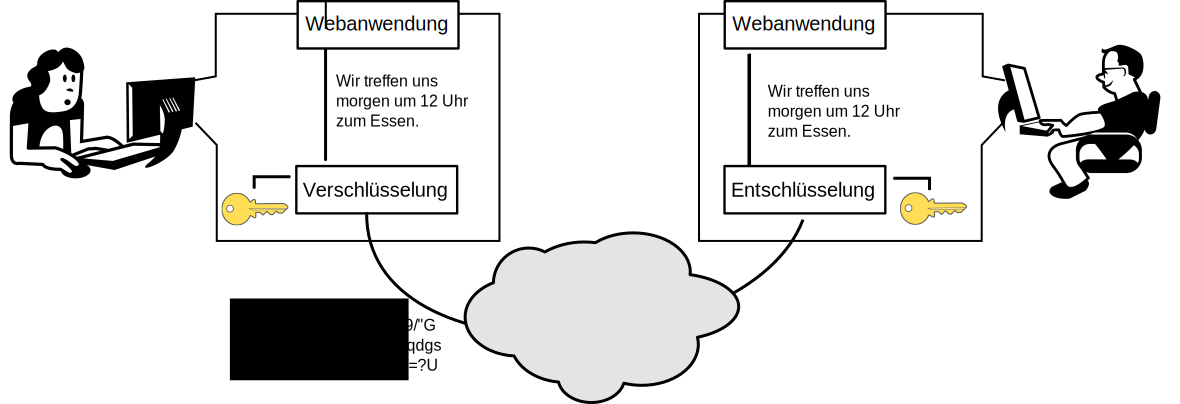
\includegraphics[width=\textwidth]{img/krypto.pdf}
    \end{center}	
\end{frame}

\begin{frame}
    \frametitle{Verschlüsselung: asymmetrisch}
    \includegraphics[height=0.7\textheight]{img/asym_encryption.png}
\end{frame}

\begin{frame}
  \frametitle{SSL}
  \begin{center}
    \only<2>{
      \includegraphics[height=0.7\textheight]{img/ssl_verified.png}
    }
    \only<3>{
      \includegraphics[height=0.7\textheight]{img/ssl_special.png}
    }
    \only<4>{
      \includegraphics[height=0.7\textheight]{img/ssl_unverified.png}
    }
  \end{center}
\end{frame}

\begin{frame}
  \frametitle{E-Mail-Selbstverteidigung}
  \begin{center}
    \includegraphics[height=0.5\textheight]{img/emailselfdefense.png}
    \begin{itemize}
      \item https://emailselfdefense.fsf.org/de/
    \end{itemize}
  \end{center}
\end{frame}

\begin{frame}
  \frametitle{Signal}
    \begin{center}
      \includegraphics[height=6cm]{img/signal1.png}
      \hspace{0.5cm}
      \includegraphics[height=6cm]{img/signal2.png}
    \end{center}
\end{frame}

\begin{frame}
  \frametitle{Alternative Dienste und Software}
  \begin{itemize}
    \item<2-> Freie Software
    \item<3-> Dezentrale Systeme
    \item<4-> Föderierte Systeme
  \end{itemize}
\end{frame}

\begin{frame}
  \frametitle{Prism Break}
  \begin{center}
    \only<1>{
      \includegraphics[height=0.5\textheight]{img/prism-break1.png}
    }
    \only<2>{
      \includegraphics[height=0.6\textheight]{img/prism-break2.png}
    }
  \end{center}
\end{frame}

\begin{frame}{Permissions}
  \begin{columns}
    \column{5.5cm}
    \footnotesize

    \textbf{Android}\\
    Einstellungen -> Apps -> Appname -> Berechtigungen ändern\\
    \vspace{0.2cm}
    Einstellungen -> Apps -> Zahnrad -> Appberechtigungen\\
    \vspace{0.5cm}

    \textbf{iOS}\\
    Einstellungen -> Privatsphäre -> Berechtigungsname\\
    \vspace{0.5cm}

    In den neuesten Versionen: Entscheidung bei erster Benutzung

    \column{5cm}

    \begin{center}
      \includegraphics[width=3.5cm]{img/permissions-android.png}
    \par\end{center}
  \end{columns}
\end{frame}

\begin{frame}
  \frametitle{TOR}
  \begin{center}
    \only<2>{
      \includegraphics[height=0.7\textheight]{img/tor1.png}
    }
    \only<3>{
      \includegraphics[height=0.7\textheight]{img/tor2.png}
    }
    \only<4>{
      \includegraphics[height=0.7\textheight]{img/tor3.png}
    }
  \end{center}
\end{frame}

\end{document}
